% Options for packages loaded elsewhere
\PassOptionsToPackage{unicode}{hyperref}
\PassOptionsToPackage{hyphens}{url}
%
\documentclass[10pt,a4paper]{article}
\usepackage[left=25mm,right=25mm]{geometry}
\usepackage{amsmath}
\usepackage{amsfonts}
\usepackage{amssymb}

\usepackage{amsmath,amssymb}
\usepackage{lmodern}
\usepackage{iftex}
\ifPDFTeX
  \usepackage[T1]{fontenc}
  \usepackage[utf8]{inputenc}
  \usepackage{textcomp} % provide euro and other symbols
\else % if luatex or xetex
  \usepackage{unicode-math}
  \defaultfontfeatures{Scale=MatchLowercase}
  \defaultfontfeatures[\rmfamily]{Ligatures=TeX,Scale=1}
\fi
% Use upquote if available, for straight quotes in verbatim environments
\IfFileExists{upquote.sty}{\usepackage{upquote}}{}
\IfFileExists{microtype.sty}{% use microtype if available
  \usepackage[]{microtype}
  \UseMicrotypeSet[protrusion]{basicmath} % disable protrusion for tt fonts
}{}
\makeatletter
\@ifundefined{KOMAClassName}{% if non-KOMA class
  \IfFileExists{parskip.sty}{%
    \usepackage{parskip}
  }{% else
    \setlength{\parindent}{0pt}
    \setlength{\parskip}{6pt plus 2pt minus 1pt}}
}{% if KOMA class
  \KOMAoptions{parskip=half}}
\makeatother
\usepackage{xcolor}
\usepackage{longtable,booktabs,array}
\usepackage{multirow}
\usepackage{calc} % for calculating minipage widths
% Correct order of tables after \paragraph or \subparagraph
\usepackage{etoolbox}
\makeatletter
\patchcmd\longtable{\par}{\if@noskipsec\mbox{}\fi\par}{}{}
\makeatother
% Allow footnotes in longtable head/foot
\IfFileExists{footnotehyper.sty}{\usepackage{footnotehyper}}{\usepackage{footnote}}
\makesavenoteenv{longtable}
\usepackage{graphicx}
\makeatletter
\def\maxwidth{\ifdim\Gin@nat@width>\linewidth\linewidth\else\Gin@nat@width\fi}
\def\maxheight{\ifdim\Gin@nat@height>\textheight\textheight\else\Gin@nat@height\fi}
\makeatother
% Scale images if necessary, so that they will not overflow the page
% margins by default, and it is still possible to overwrite the defaults
% using explicit options in \includegraphics[width, height, ...]{}
\setkeys{Gin}{width=\maxwidth,height=\maxheight,keepaspectratio}
% Set default figure placement to htbp
\makeatletter
\def\fps@figure{htbp}
\makeatother
\setlength{\emergencystretch}{3em} % prevent overfull lines
\providecommand{\tightlist}{%
  \setlength{\itemsep}{0pt}\setlength{\parskip}{0pt}}
\setcounter{secnumdepth}{-\maxdimen} % remove section numbering
\ifLuaTeX
  \usepackage{selnolig}  % disable illegal ligatures
\fi
\IfFileExists{bookmark.sty}{\usepackage{bookmark}}{\usepackage{hyperref}}
\IfFileExists{xurl.sty}{\usepackage{xurl}}{} % add URL line breaks if available
\urlstyle{same} % disable monospaced font for URLs
\hypersetup{
  hidelinks,
  pdfcreator={LaTeX via pandoc}}

\author{}
\date{}



\usepackage{listings}
\usepackage{color}

\definecolor{dkgreen}{rgb}{0,0.6,0}
\definecolor{gray}{rgb}{0.5,0.5,0.5}
\definecolor{mauve}{rgb}{0.58,0,0.82}

\lstset{frame=tb,
  language=C,
  aboveskip=3mm,
  belowskip=3mm,
  showstringspaces=false,
  columns=flexible,
  basicstyle={\small\ttfamily},
  numbers=none,
  numberstyle=\tiny\color{gray},
  keywordstyle=\color{blue},
  commentstyle=\color{dkgreen},
  stringstyle=\color{mauve},
  breaklines=true,
  breakatwhitespace=true,
  tabsize=3
}

\usepackage{multicol}
\usepackage{graphicx}
\usepackage{epstopdf}

\epstopdfDeclareGraphicsRule{.gif}{png}{.png}{convert gif:#1 png:\OutputFile}
\AppendGraphicsExtensions{.gif}
\usepackage{chngcntr}
\counterwithin*{equation}{section}
\counterwithin*{equation}{subsection}

\usepackage{float} 

\usepackage{amsmath}
\let\oldsubsection\subsection
\renewcommand{\subsection}{%
    \setcounter{equation}{0}%
    \oldsubsection%
}

\begin{document}


\begin{flushleft}
\begin{LARGE}EE 435 Homework 3 Spring 2024
\end{LARGE}
\\Jonathan Hess
\\\href{https://github.com/Jetsama/EE435/tree/main/HW3}{GitHub Page}
\end{flushleft}

\section{Assumptions}
In the following problems, if reference to a semiconductor process is needed, assume
processes with characteristics: CMOS Process -- $\mu_n$COX=100$\mu$A/v2 , $\mu_n$pCOX=33$\mu$A/v2 ,
VTNO=0.5V,
 VTPO= - 0.5V,
  COX=2fF/$\mu^2$,
   $\mu_n$= $\mu_p$= 0.01V-1,
    and $\upsilon$= 0.4 V-1/2

\section{Problem 1}
\begin{quote}
Consider the following quarter circuit. Assume an engineer from
Samswrong has proposed this as the quarter circuit for building an operational amplifier
with current-mirror connected counterpart circuits, n-channel inputs, and a tail current
bias.\\
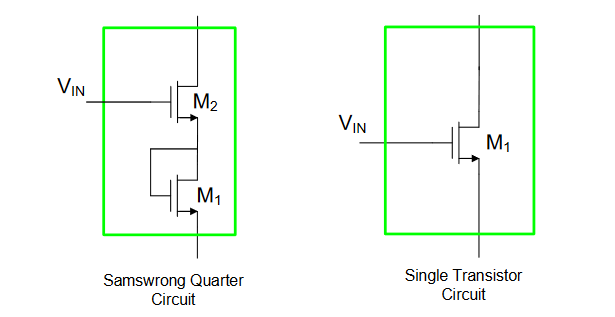
\includegraphics[width=3in]{images/Problem1.png} \\
\end{quote}

\subsection{Problem 1a}
\begin{quote}

Determine the two-port model of the Samswrong Quarter Circuit in terms of the small-signal model parameters\\

\end{quote}



\subsection{Problem 1b}
\begin{quote}

Create the differential input operational amplifier described above and determine the differential voltage gain and the GB in terms of the small-signal parameters.small-
\end{quote}





\subsection{Problem 1c}
\begin{quote}

Repeat part b) but express in terms of the practical design parameters
\end{quote}



\section{Problem 2}
\begin{quote}
Consider again the amplifier in Problem 1. Assume the Samswrong
engineer made the argument that the operational amplifier formed with the Samswrong
quarter circuit is superior to that of the reference op amp (that was derived from the
single-transistor quarter circuit). To draw this conclusion, the engineer designed both
circuits with a 1 mW power budget and chose VEB1 and VEB2 for the Samswrong quarter
circuit both be 150 mV and VEB1 for the reference op amp to be 500 mV. With these
two designs, the engineer argued that the op amp derived from the Samswrong quarter
circuit offered an improvement in both dc gain and GB.
\end{quote}

\subsection{Problem 2a}
\begin{quote}
Are there improvements in both gain and GB actually achieved with the
Samswrong op amp?\\
\end{quote}


\subsection{Problem 2b}
\begin{quote}
Is the comparison of the two structures fair?\\
\end{quote}


\subsection{Problem 2c}
\begin{quote}
Make your own comparison of the two operational amplifiers.\\
\end{quote}




\section{Problem 3}
\begin{quote}
Consider an operational amplifier with differential inputs using the n-
channel cascode structure for the quarter circuit and the Wilson Current Mirror
(converted to p-channel devices) as an alternative counterpart circuit (the Modified
Wilson Current Mirror was introduced in Lecture 6).\\
\end{quote}

\subsection{Problem 3a}
\begin{quote}
Give the circuit schematic of the operational amplifier if it is biased with a tail
current source.
\end{quote}

\subsection{Problem 3b}
\begin{quote}
If a capacitive load of value CL is placed on the output, determine the differential
voltage gain Ad(s) for this op amp.
\end{quote}

\subsection{Problem 3c}
\begin{quote}
Determine the dc voltage gain and the GB for the op amp in terms of the small-
signal model parameters.
\end{quote}


\subsection{Problem 3d}
\begin{quote}
Make a comparison of the performance of this circuit with that of the telescopic
cascode operational amplifier where the counterpart circuit of the telescopic
cascode amplifier is connected as a current mirror.
\end{quote}




\section{Problem 4}
\begin{quote}
Consider the folded-cascode operational amplifier with n-channel inputs, a
tail current bias, and a current-mirror connected counterpart circuit. Assume it has been
designed with a VDD=2V supply voltage, all devices were designed to have VEB=200 mV,
the power dissipation was set at 10 mW, and the tail current of the differential pair at the
input was 1/3 of the current coming out of VDD.
\end{quote}


\subsection{Problem 4a}
\begin{quote}
Give the circuit schematic of this operational amplifier
\end{quote}


\subsection{Problem 4b}
\begin{quote}
Give the device dimensions (W/L values) for all devices in the circuit.
\end{quote}


\subsection{Problem 4c}
\begin{quote}
Numerically give the dc voltage gain and the GB for this op amp
\end{quote}



\section{Problem 5}
\begin{quote}
In some processes, transistors with several different threshold voltages are
available. Assume M1 and M2 in the circuit below have threshold voltages of VT1 and
VT2 but all other model parameters are the same. Assume VT1=VDD/5 and VT2=VDD/10.
\end{quote}

\subsection{Problem 5a}
\begin{quote}
Obtain the two-port model for this device.
\end{quote}



\subsection{Problem 5b}
\begin{quote}
Identify a “practical” design parameter domain for this device
\end{quote}

There is a practical parameter IQ which is the current flowing through the transistors at the quiescent point.

\subsection{Problem 5c}
\begin{quote}
Give the schematic of a fully-differential operational amplifier with tail
current bias if this is used as the “Quarter Circuit” for the op amp.
\end{quote}



\subsection{Problem 5d}
\begin{quote}
What is the dc voltage gain and the GB of the operational amplifier of part c)?
Assume a load capacitor of CL on both outputs.
\end{quote}

\section{Problem 6}
\begin{quote}
The telescopic cascode op amp with n-channel inputs is shown below.
\end{quote}
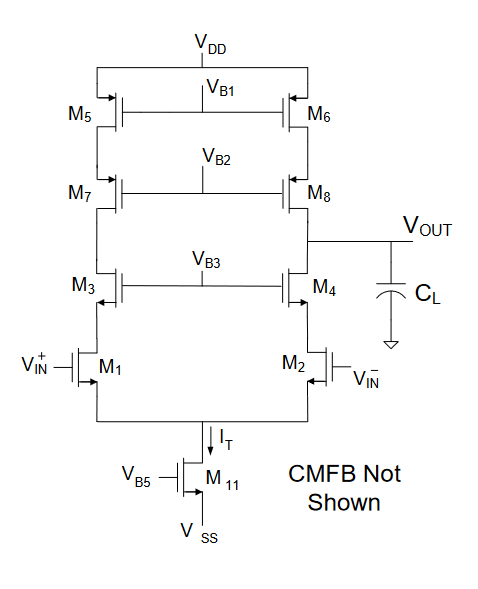
\includegraphics[width=3in]{images/Problem6.png} \\

\subsection{Problem 6a}
\begin{quote}
Determine the common-mode gain of the telescopic cascode op amp if the tail
current source is ideal.
\end{quote}

\subsection{Problem 6b}
\begin{quote}
Give the circuit schematic for the telescopic cascode op amp with p-channel
inputs
\end{quote}



\subsection{Problem 6c}
\begin{quote}
Determine the positive and negative slew rates of the amplifer shown if the tail
current source is ideal with a current of 100uA and the load capacitor is 2pF.
\end{quote}






\begin{thebibliography}{9}
\bibitem{opamp}\href{https://ieeexplore.ieee.org/document/9532225}{Design and Analysis of Two-Stage CMOS Operational Amplifier for Fluorescence Signal Processing}
\bibitem{opamp-pics}\href{https://www.electronics-tutorials.ws/opamp/opamp_1.html
}{Operational Amplifier Basics}
\bibitem{patent}\href{https://github.com/Jetsama/EE435/blob/main/HW1/Sources/US20230051462A1.pdf}{TI Patent:Differential Amplifier Common Mode Voltage}
\bibitem{GFS}\href{https://en.wikipedia.org/wiki/Google_File_System}{Wikipedia: Google File System}

\end{thebibliography}

\end{document}
